\chapter{Image recognition for IBD reconstruction with the SPMT system}
\label{sec:jcnn}

\epigraph{\textit{Dave} - Give me the position and momentum, HAL. \\
\textit{HAL} - I'm afraid I can't do that Dave. \\
\textit{Dave} - What's the problem ? \\
\textit{HAL} - I think you know what the problem is just as well as I do. \\
\textit{Dave} - What are you talking about, HAL? \\
\textit{HAL} - $\sigma_x \sigma_p \geq \frac{\hbar}{2}$}

As explained in chapter \ref{sec:juno}, JUNO is an experiment composed of two systems, the Large Photomultiplier (LPMT) and the Small Photomultiplier (SPMT). Both of the system observe the same physics event inside of the same medium but they differ in their photo-coverage, respectively 75.2\% and 2.7\%, their dynamic range (see section \ref{sec:juno:LPMT}, a thousands versus a few dozen, and their front-end electronics (see section \ref{sec:juno:LPMT}).

They are complementary in their strengths and weaknesses and support each other. One important point is their differences in expected resolution, the LPMT system outperform largely the SPMT system but is subject to effects such as charge  non linearity \cite{juno_collaboration_calibration_2021} that could bias the reconstruction, effect that the SPMT system is impervious to. This topic will be studied in more detail in chapter \ref{sec:joint_fit}. Also, due to the dynamic range of the LPMT, in case of high energy and high density event such as core-collapse supernova, the LPMT system could saturate and the lower photo-coverage become a benefit.

Thus, although event reconstruction algorithm and physics analysis combines both LPMT and SPMT systems, individual approach are key studies to understand the detector and ensure their reliability. This topic will also be studied in more details in chapter \ref{sec:joint_fit}. The subject of this chapter is to propose a machine learning algorithm for the SPMT reconstruction based on Convolutional Neural Network (CNN).

\section{Motivations}

% -------------- Plan for motivation section ----------------
%\begin{itemize}
%  \item Promise of machine learning -> Exploit raw data
%  \item Victor already done reco for SPMT
%  \item Can CNN give similar results ? Better results ?
%  \item Multiple reco methods good for reconstruction
%  \item Comparison, difference in behavior
%\end{itemize}

As explained in chapter \ref{sec:ml}, Machine Learning (ML) algorithms shine when modeling highly dimensional data from a given dataset. In our case, we have access to complete monte-carlo simulation of our detector to produce arbitrary large datasets that could represent multiple years of data taking.
Ideally ML algorithms would be able to consider the entirety of the information in the detector and converge on the best parameters to yield optimal results, while classical methods where the algorithms could be biased by the prior knowledge of the detector and physics processes. To study this potential phenomena, we will compare our machine algorithm to a classical reconstruction method developed for energy and vertex reconstruction \cite{lebrin_towards_2022}.

We have access to a very detailed simulation of the detector (section \ref{sec:juno:software}) that will allow us to simulate arbitrary large dataset of data while giving access to the all the physics parameters of the event. Those parameters include the target of our reconstruction algorithms: the vertex and position at with the event happened. As introduced above, we hope that the ML algorithm will be able to used all the informations in the event, meaning that potential mismodelings in our simulation could be exploited by the algorithm. This specific subject will be studied in chapter \ref{sec:janne}.

\section{Method and model}
% --------------- Plan for method and model -----------------
%\begin{itemize}
%  \item JUNO is an array of sensor following a quasi uniform and istropic geometric repartition -> Basically pixels -> Image
%  \item CNN is gud for image processing (cite a lot of things)
%  \item Details the architecture (Inspired from VGG 16)
%    \begin{itemize}
%      \item Convolutional layers
%      \item Pooling layers -> Twice the channels when pooling by 2 -> Keep the same "amount" of information
%      \item Dropout (introduce overtraining, maybe introduce overfitting in ML chapter ?)
%      \item Vectorization fed to FCDNN
%    \end{itemize}
%\end{itemize}

One of simplest way to look at JUNO data is to consider the detector as an array of geometrically distributed sensors on a sphere. Their repartition is almost homogeneous, on this sphere surface providing an almost equal amount of information per unit surface on this sphere. It is then tempting to represent the detector as a spherical image with the PMT in place of pixel. Two events with two different energy or position would produce two different images.

The most common approach in machine learning for image processing and image recognition is the Convolutional Neural Network (CNN). It is widely used in research and industry \cite{simonyan_very_2015, ciresan_multi-column_2012, abbasi_convolutional_2021, maksimovic_cnns_2021} due to its strengths (see section \ref{sec:ml:cnn}) and has proven its relevance in image processing.

Some CNN are developed to process spherical images \cite{cohen_spherical_2018} but for the sake of simplicity and as a first approach we decided to go with a planar projection of the detector, approach that has proven its efficiency using the LPMT system (see section \ref{sec:juno:ml}). The details about this planar projection will be discussed in section \ref{sec:jcnn:data}.

\begin{figure}[ht]
  \centering
  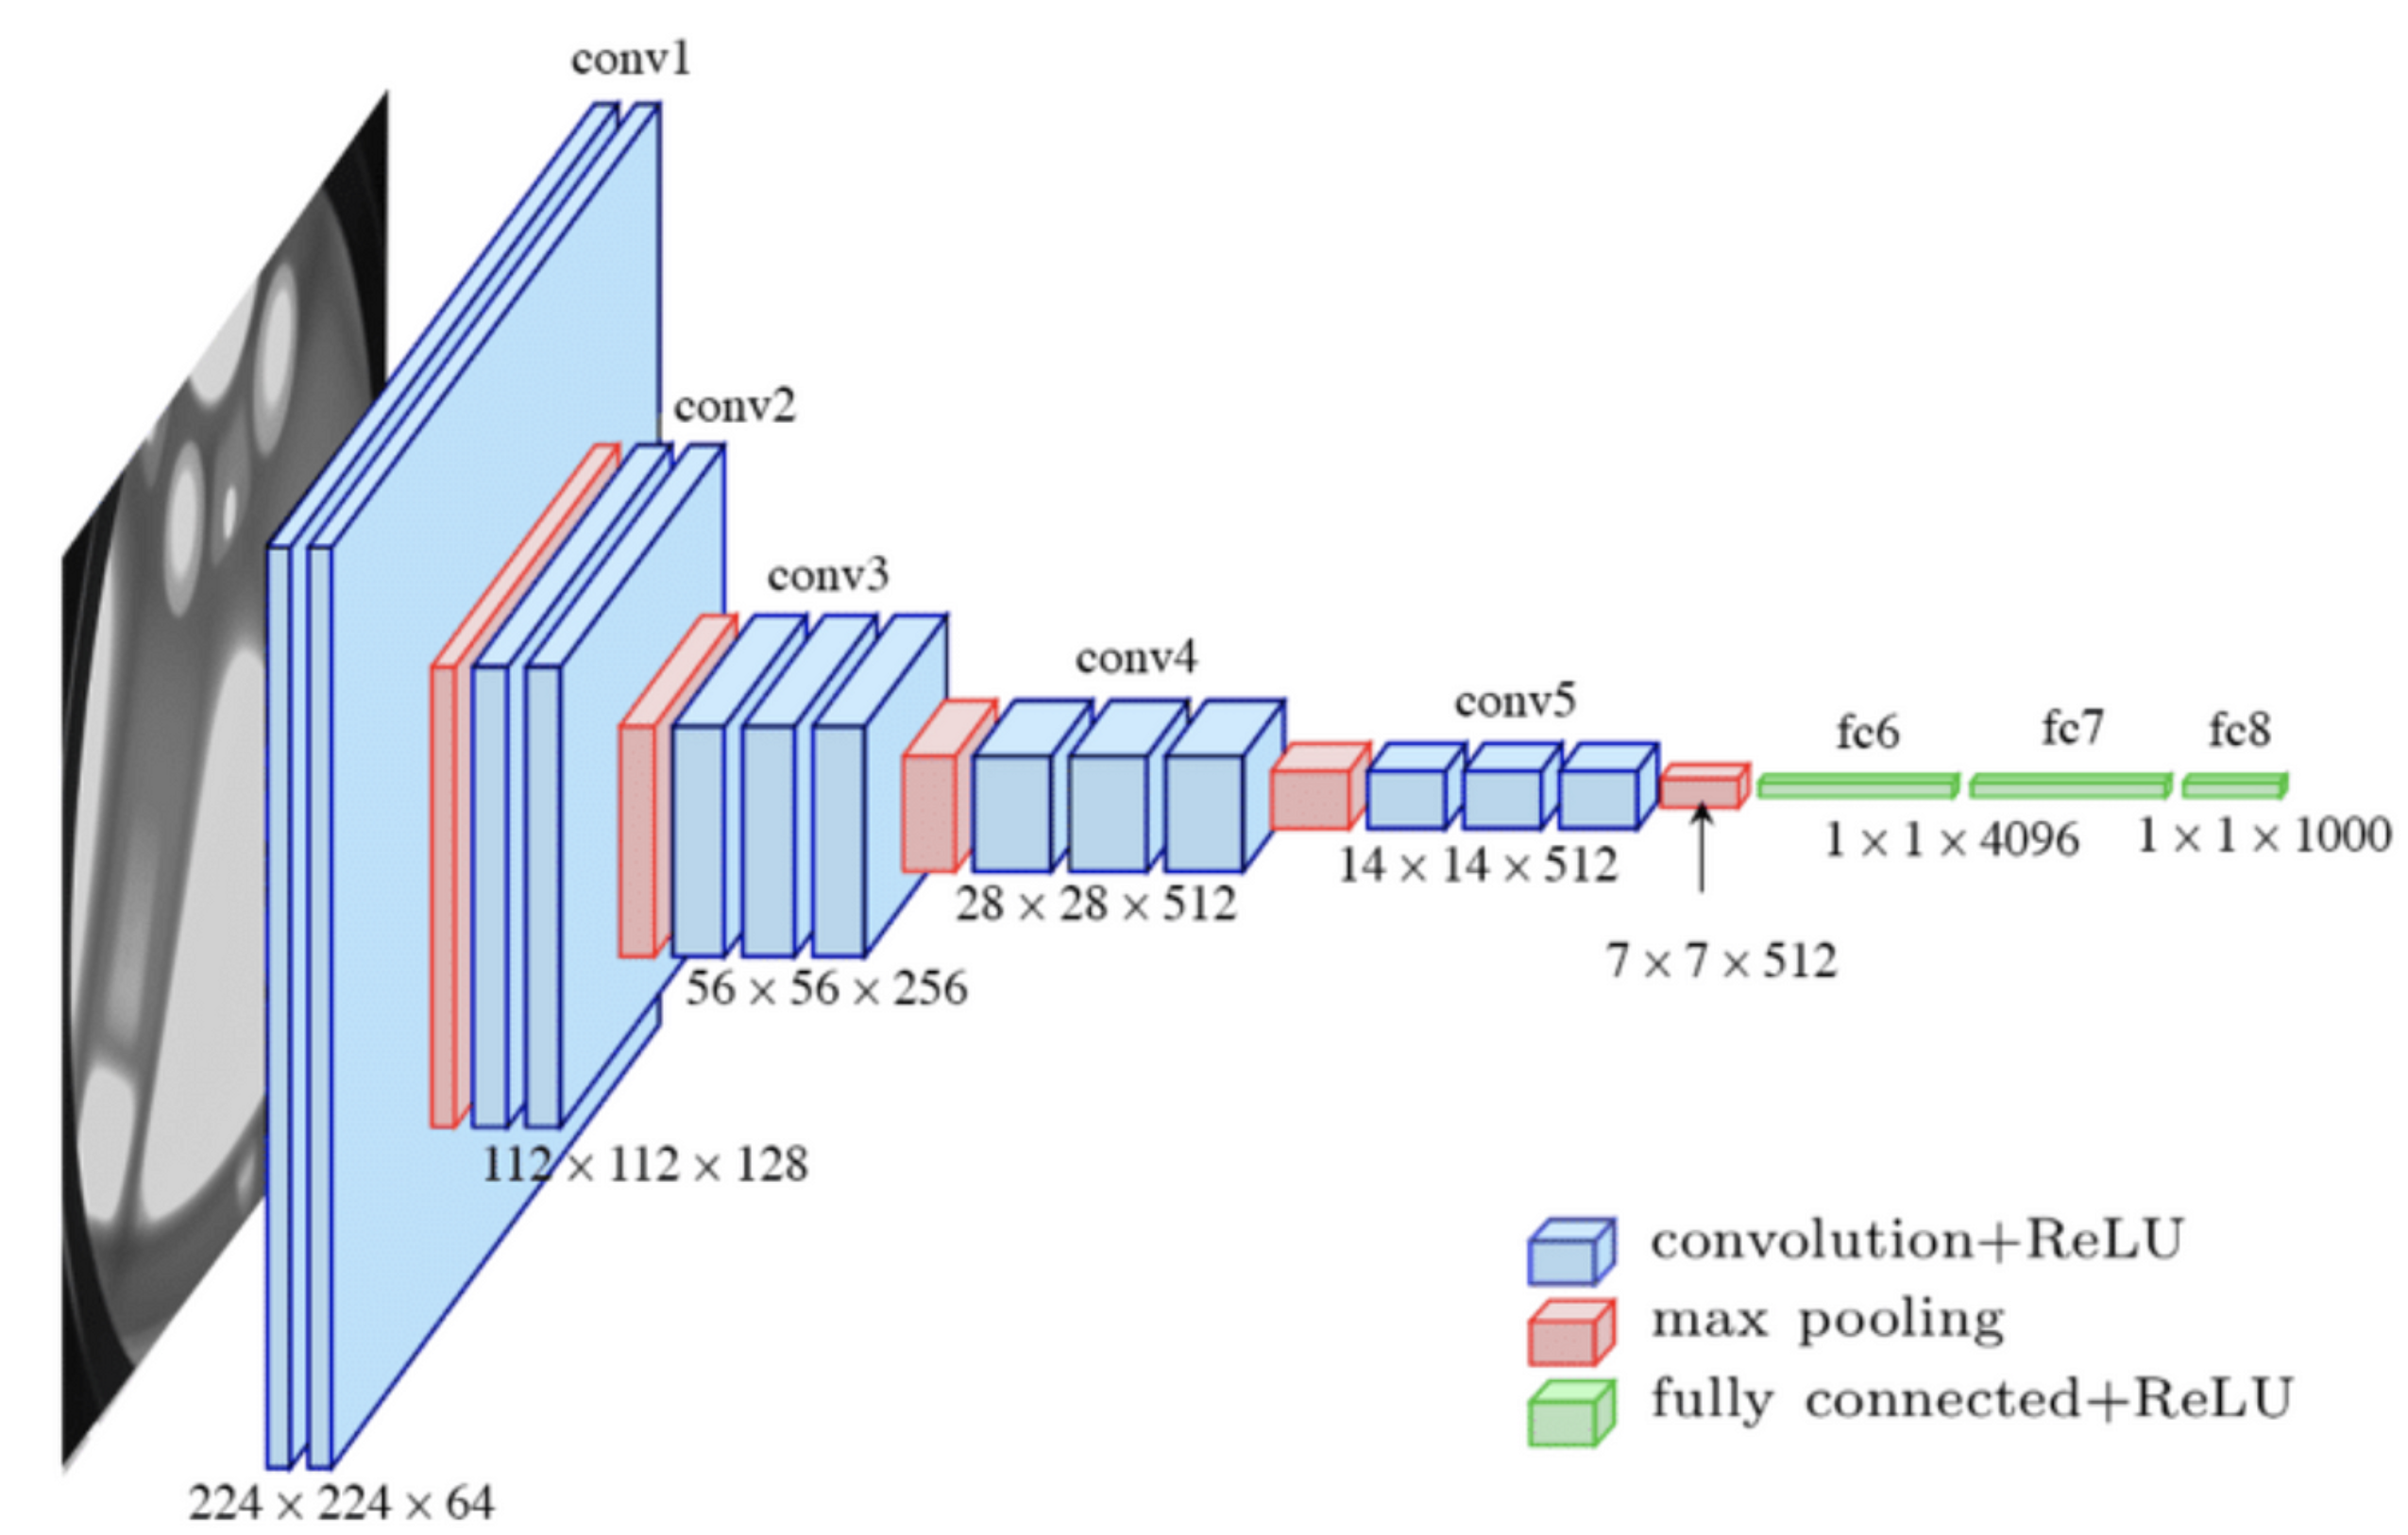
\includegraphics[height=6cm]{images/jcnn/vgg16.png}
  \caption{Graphic representation of the VGG-16 architecture, presenting the different kind of layer composing the architecture.}
  \label{fig:jcnn:vgg16}
\end{figure}

\subsection{Model}
\label{sec:jcnn:model}

The architecture we use is derived from the VGG-16 architecture \cite{simonyan_very_2015} illustrated in figure \ref{fig:jcnn:vgg16}. We define a set of hyperparameters that will define the size, complexity and computational power of the NN. The chose hyperparameters are detailed below and their values are presented in table \ref{tab:jcnn:hyper}.
\begin{itemize}
  \item $\mathbf{N_{blocks}}$: the number of convolution blocks, a block being composed of two convolutional layers with $3\times3$ filters using ReLU activation function, a $3\times3$ max-pooling layer (except for the last block) and a dropout layer.
  \item $\mathbf{N_{channels}}$: The number of channels in the first block. The number of channels in the subsequent blocks are calculated using $N^i_{channels} = 2^{i} * N_{channels}, i \in [1..N_{blocks}]$.
  \item \textbf{FCDNN configuration}: The result of the last convolution layer is flattened then fed to a FCDNN. Its configuration is expressed as a sequence of fully connected linear layer using the PReLU activation function. For example $2 * 1024 + 2 * 512$ is the sequence of 2 layers with a width of 1024 followed by 2 other layers with a width of 512. Finally the last layer is a 4 neurons wide linear layers without activation function. Each neurons of the last layer represent a component of the interaction vertex: Energy, X, Y, Z.
  \item \textbf{Loss}: The loss function. In this work we study two different loss function $(E+V)$ and $(E_r + V_r)$ detailed below.
\end{itemize}


We explore in this work two different activation functions
\begin{align}
  (E+V)(E, x, y, z) &= \bigg\langle (E - E_{true})^2 + 0.85 \sum_{\lambda \in [x, y, z]} (\lambda - \lambda_{true})^2 \bigg\rangle \\
  (E_r + V_r)(E, x, y, z) &=  \bigg\langle \frac{(E - E_{true}) ^ 2}{E_{true}} + \frac{10}{R} \sum_{\lambda \in [x, y, z]} (\lambda - \lambda_{true})^2 \bigg\rangle
\end{align}
where $R$ is the radius of the CD. With the energy in MeV and the distance in meters, we use the factor 0.85 and 10 to equilibrate the two term of the loss function so they have the same magnitude.
\begin{itemize}
  \item The loss function $(E+V)$ is close to a simple Mean Squared Error (MSE). MSE is one of the most basic loss function, the derivative is simple and continuous in every point. It is a strong starting point to explore the possibility of CNNs.
  \item $(E_r + V_r)$ can be see as a relative MSE.
\end{itemize}
The idea is that: due to the inherent statistic uncertainty over the number of collected Number of Photo Electrons (NPE), the absolute resolution $\sigma (E - E_{true})$ will be larger at higher energy than at low energy. But we expect the \textit{relative} energy resolution $\frac{\sigma(E - E_{true})}{E_true}$ to be smaller at high energy than lower energy as illustrated in figure \ref{fig:juno:rec:qtmle}. Because of this, by using simple MSE the most important part in the loss come from the high energy part of the dataset whereas with a relative MSE, the most important become the low energy events in the dataset. We hope that by using a relative MSE, the neural network will focus on low energy events where the reconstruction is considered the hardest part of the dataset.


\begin{table}[ht]
  \centering
  \begin{tabular}{ | c | c | }
    \hline $N_{blocks}$ & \{2, 3, 4\} \\
    \hline $N_{channels}$ & \{32, 64, 128\} \\
    \hline
    \multirow{4}{*}{FCDNN configurations} & 2 * 1024 \\
                                        & 2 * 2048 + 2 * 1024 \\
                                        & 3 * 2048 + 3 * 512 \\
                                        & 2 * 4096 \\
    \hline
    Loss & \{$E+V$, $E_r + V_r$\} \\
    \hline
  \end{tabular}
  \caption{Sets of hyperparameters values considered in this study}
  \label{tab:jcnn:hyper}
\end{table}

Each combination of those hyperparameters (for example $(N_{blocks} = 2, N_{channels} = 32, \mathrm{FCDNN} = (2 * 1024), \mathrm{Loss} = (E+V))$), subsequently designated as configurations, is then tested and compared to each other over an analysis sample. We cannot use the mean loss because we consider multiple loss functions, there is no guarantee that comparison of their numerical value will be meaningful. We use multiple observables to rank the performances of each configuration:
\begin{itemize}
  \item The mean absolute energy error $\langle E \rangle = \langle | E - E_{true} | \rangle$. It is an indicator of the energy bias of our reconstruction.
  \item The standard deviation of the energy error $\sigma E = \sigma (E - E_{true})$. This the indicator on our precision in energy reconstruction.
  \item The mean distance between the reconstructed vertex and the true vertex $\langle V \rangle = \langle | \vec{V} - \vec{V}_{true} | \rangle$. This an indicator of the bias and precision of our vertex reconstruction.
  \item The standard deviation of the distance between the true and reconstructed vertex $\sigma V = \sigma |\vec{V} - \vec{V}_{true}|$. This is an indicator if the precision in our vertex reconstruction.
\end{itemize}


%Indeed, let's say we consider error on each of the component as random variable following a normal distribution. We allow ourself to use this representation as our signal possess a strong statistical uncertainty in NPE that follow a Poisson law, i.e. a Gaussian law $\mathcal{N}$ when NPE is high enough which is the case for our signal. So following:
%\begin{equation}
%  \Delta V = |\vec{V} - \vec{V}_{true}| = \sqrt{\Delta X^2 + \Delta Y^2 + \Delta Z^2}; ~ \Delta X, \Delta Y, \Delta Z \sim \mathcal{N}
%\end{equation}
%then
%\begin{equation}
%  \Delta V \sim \chi
%\end{equation}
%where $\chi$ is a Chi law which probability density function is different from 0 only in $\mathbb{R}^+$

\subsection{Data representation}
\label{sec:jcnn:data}
%\begin{itemize}
%  \item Data is 240x240 images
%    \begin{itemize}
%      \item Following $\theta$ and $\phi$ distribution, explain the coordinate system of JUNO
%      \item Optimized for $\approx$ 1 SPMT/pixel
%      \item 1 Charge channel
%      \item 1 Time channel
%    \end{itemize}
%  \item Discuss data format
%    \begin{itemize}
%      \item Empty pixel ? -> $Q = 0$, $T = 0$, what does it means/says ? 0 = no signal in a way
%      \item Image distortion
%        \begin{itemize}
%          \item \textbf{Maybe speak of this in the conclusion ?} Could be done in two step:
%          \item 1. Reconstruct $\theta$ and $\phi$
%          \item 2. "Rotate" the image so the event is at the center of the image -> Prevent distortion + reconstruction E and R become pseudo rotational invariant (as they should be)
%        \end{itemize}
%    \end{itemize}
%\end{itemize}

This data is represented as $240 \times 240$ images, equivalent to third order tensor, with a charge $Q$ channel and a time $t$ channel. The SPMTs are then projected on the plane as illustrated in figure \ref{fig:jcnn:pmt_rep}. The $x$ position is proportional to $\theta$ and the $y$ position is defined by $\phi \sin{\theta}$ in spherical coordinates. $\theta = 0$ is defined as being the top of the detector and $\phi = 0$ is defined as an arbitrary direction in the detector. In practice, this is the $\phi = 0$ given by the MC simulation.

\begin{align}
  x &= \bigg\lfloor \frac{\theta \cdot H}{\pi} \bigg\rfloor, ~ \theta \in [0, \pi] \\
  y &= \bigg\lfloor \frac{(\phi + \pi) \sin{\theta} \cdot W}{2\pi}\bigg\rfloor, ~ \phi \in [-\pi, \pi], ~ \theta \in [0, \pi]
\end{align}
where $H$ is the height of the image, $W$ the width of the image and $(0,0)$ the top left corner of the image.

When two SPMTs are in the same pixel, the charges are summed and the lowest of the hit-time is chosen. The SPMTs being located close to each other, we expect the time difference between two successive physics signals, two photons being collected, to be small. The first hit time is chosen because it can be considered as the relative propagation time of the photons that went the "straightest", i.e. that went under the less perturbation of the two. The only potential problem in using this first time come from the Dark Noise (DN). Its time distribution is uniform over the signal and could come before a signal hit on the other SPMT in the pixel. In that case, the time information in the pixel become irrelevant and we lose the timing information for this part of the detector.
As illustrated in figure \ref{fig:jcnn:pmt_rep} the dimension have been chosen optimized so that at most two SPMTs are in the same pixel while keeping the number of empty pixels relatively low to prevent this kind of issue.

While it could be possible to use larger images (more pixel) to prevent overlapping, keeping image small images gives multiple advantages:
\begin{itemize}
  \item As presented in section \ref{sec:jcnn:model}, the convolution filter we use are $3 \times 3$ convolution filter, meaning that if SPMTs would be separated by more that one pixel, the first filter would only see one SPMT per filter. This behavior would be kind of counterproductive as the first convolution block would basically be a transmission layer and would just induce noise in the data.
  \item It keep the network relatively small, while this do not impact the convolution layers, the flatten operation just before the FCDNN make the number parameters in the first layer of it dependent on the size of the image.
  \item It reduce the number of empty pixel in the image.
\end{itemize}
The question of empty pixel is an important question in this data representation. Their is two kind of empty pixel in the data.

The first kind is pixel that contain a SPMT but the SPMT did not get hit nor registered any dark noise during the event. In this case, the charge channel is zero, which have a physical meaning but then come the question of the time layer. One could argue that the correct time would be infinity (or the largest number our memory allows us) because the hit ``never'' happened, so extremely far from the time of the event. This cause numerical problem as large number, in the linear operation that are happening in the convolution layers, are more signifiant than smaller value. We could try to encode this feature in another way but no number have any significance due to our time being relative to the trigger of the experiment so $-1$ for example is out of question. Float and Double gives us access to special value such as NaN (Not a Number) \cite{noauthor_ieee_2019} but the behavior is to propagate the NaN which leaves us with NaN for energy and position. We choose to keep the value 0 because it's the absorbing element of multiplication, absorbing the ``information'' of the parameter it would be multiplied by. It also can be though as no activation in the ReLU activation function.

The second kind of pixel is pixel that do not represent parts of the detector such as the corners of the images. The question is basically the same, what to put in the charge and the time channel. The decision is to set the charge and time at 0 following the reasoning presented above. Its important to keep in mind that the fact that a part of the detector that has not been hit is also an information: There is no signal in this part of the detector. This problematic will be explored in more details in chapter \ref{sec:jgnn}.

Another problematic that happens with this representation, and this is not dependent of the chosen projection, is the deformation in the edges of the image and the loss of the neighbouring information in the for the SPMTs at the edge of the image $\phi \sim 180^\circ$. This deformation and neighbouring loss could be partially circumvented as explained in section \ref{sec:jcnn:prospect}

\subsection{Dataset}
% 1 Millions MC e+ events for training (900k for train, 50k for validation and 50k for test)
%   \begin{itemize}
%     \item MC for the moment, will need to retrain with mix of calibration data (Good question, is the CNN PID agnostic ?)
%     \item 47 IBD/day -> 1M event is 21k days of data (for reference, 6 years of data is 94k events)
%     \item Events are "optimistic"
%       \begin{itemize}
%         \item No pile-up
%         \item w/o neutrons
%         \item time window is decided by electronics
%       \end{itemize}
%   \end{itemize}


In this study we use one million events coming from the full JUNO official monte-carlo simulations J23.0.1-rc8.dc1 (released the 7th January 2024). To put in perspective, the expected IBD rate in JUNO is 47 / days. Taking into account the calibration time, and the source reactor shutdown, it amount to $\sim 94'000$ IBD events in 6 years. With this million of event, we are training the equivalent of $\sim 10$ years of data. With this amount we reach a density of $4783 \frac{\mathrm{event}}{\mathrm{m}^3\cdot\mathrm{MeV}}$, meaning our dataset is representative of the multiple event scenarios that could be happening in the detector.

While we expect and hope the monte-carlo simulation to give use a realistic representation of the detector, there could be effect, even after the fine-tuning on calibration data, that the simulation cannot handle. Thus, once the calibration will be available, we will need to evaluate, and if needed retrain, the network on calibration data to establish definitive performances.

The data used during this analysis is monte carlo data using the official JUNO simulation software (see section \ref{sec:juno:software} for details). The simulated data is composed of positron events, uniformly distributed in the CD volume and in kinetic energy over $E_k \in [0; 9]$ MeV producing a deposited energy $E_{dep} \in [1.022; 10.022]$ MeV. This is done to mimic the signal produced by the IBD prompt signal. Uniform distribution are used so that the CNN does not learn a potential energy distribution, favoring some part of the energy spectrum instead of other.

Those events can be considered as ``optimistic'' as there is no pile-up with potential background or other IBD.

The dark noise and time window come from the monte-carlo simulation of the electronic and trigger system. The dark noise rate used in this study is coming from studies and calibration of the PMTs outside of the experimental setup \cite{cao_mass_2021, abusleme_mass_2022}.


\subsection{Data characteristics}
%TODO: Faire un bestiaire de diofferents type d'event

\begin{figure}[ht]
  \centering
  \begin{subfigure}[b]{0.48\textwidth}
    \centering
    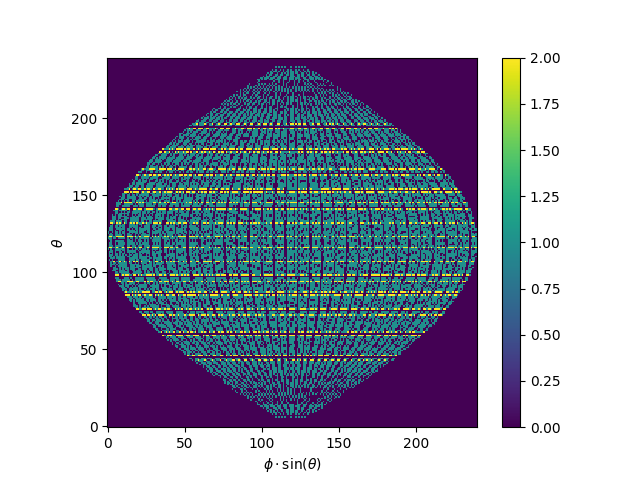
\includegraphics[width=\textwidth]{images/jcnn/pmt_repartition.png}
    \caption{Repartition of SPMTs in the image projection. The color scale is the number of SPMTs per pixel}
    \label{fig:jcnn:pmt_rep}
  \end{subfigure}
  \hfill
  \begin{subfigure}[b]{0.48\textwidth}
    \centering
    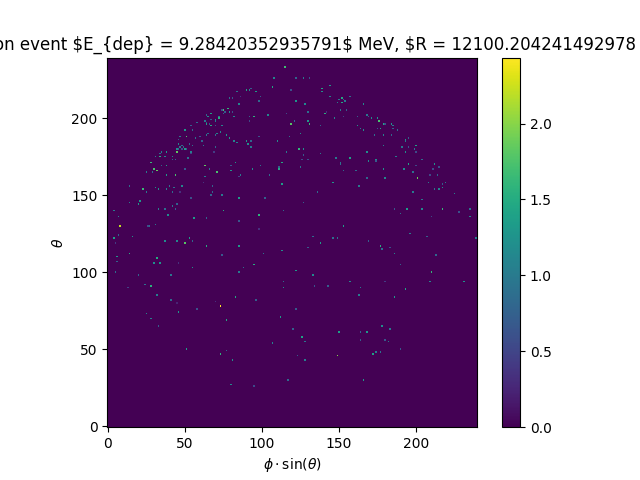
\includegraphics[width=\textwidth]{images/jcnn/illustration_event.png}
    \caption{Example of the charge channel of an event as seen by the CNN \textbf{(Need to redo the title)}}
    \label{fig:jcnn:event_example}
  \end{subfigure}
  \caption{}
\end{figure}

\section{Results}

Before presenting the results, lets discuss the different observables.

The event are considered point like in this study. The target truth position, or vertex, is the mean position of the energy deposits of the positron and the two annihilation gammas. Due to the symmetries of the detector, we mainly considered and discuss the bias and precision evolution depending of the radius $R$ but we will still monitor the performances depending of the spheric angle $\theta$ and $\phi$. From the detector construction and effect we expect relative important dependencies in radius thanks to the TR area effect presented in section \ref{sec:juno:reco} and the possibility for the positron or the gammas to escape from the CD for near the edge events. We  also expect dependence in $\theta$, the top of the experiment being non-instrumented due to the filling chimney. It is also to be noted that the events in the dataset are uniformly distributed in the CD, and so are uniformly distributed in $R^3$ and $\phi$. The $\theta$ distribution is not uniform and we will have more event for $\theta \sim 90^{\circ}$ that $\theta \sim 0^{\circ}$ or $\theta \sim 180^{\circ}$.

We define multiple energy in JUNO:
\begin{itemize}
  \item $E_\nu$: The energy of the neutrino.
  \item $E_k$: The kinetic energy of the resulting positron from the IBD.
  \item $E_{dep}$: The deposited energy of the positron and the two annihilation gammas.
  \item $E_{vis}$: The equivalent visible energy, so $E_{dep}$ after the detector effect such as the absorption of scintillation photons by the LS and the LS response non-linearity.
  \item $E_{rec}$: The reconstructed energy by the reconstruction algorithm. The expected value depend on the algorithm we discuss about. For example the algorithm presented in section \ref{sec:juno:reco} is reconstructing $E_{rec}$ while the ones presented in section \ref{sec:juno:ml} reconstruct $E_{dep}$.
\end{itemize}

In this study, we will set $E_{rec}$ as our target for energy reconstruction. This choice is motivated by the ease with which we can retrieve this information in the monte-carlo data while $E_{vis}$  is less trivial to retrieve.


%\begin{itemize}
%  \item We want to reconstruct the E from $\bar{\nu_e}$
%  \item Difference between multiple E -> $E_{vis}$, $E_{rec}$, $E_k$
%  \item Comparison with victor results
%  \item \textbf{More details when I'll look into the retrained data}
%  \item Discuss of the differences
%  \item Discuss of the principle of error decorelation
%    \begin{itemize}
%      \item Possible improvements
%      \item Combining algorithms
%      \item Average sum
%    \end{itemize}
%\end{itemize}

\section{Prospect}
\label{sec:jcnn:prospect}

\section{Conclusion}
Intoduction next chapter
